%%%%%%%%%%%%%%%%%%%%%%%%%%%%%%%%%%%%%%%%%
% Beamer Presentation
% LaTeX Template
% Version 1.0 (10/11/12)
%
% This template has been downloaded from:
% http://www.LaTeXTemplates.com
%
% License:
% CC BY-NC-SA 3.0 (http://creativecommons.org/licenses/by-nc-sa/3.0/)
%
%%%%%%%%%%%%%%%%%%%%%%%%%%%%%%%%%%%%%%%%%

%----------------------------------------------------------------------------------------
%	PACKAGES AND THEMES
%----------------------------------------------------------------------------------------

\documentclass{beamer}
\usepackage{xcolor}
\usepackage{lmodern}
\usepackage[ruled,vlined]{algorithm2e}
\usepackage{subcaption}
\usepackage{appendixnumberbeamer}

\mode<presentation> {

% The Beamer class comes with a number of default slide themes
% which change the colors and layouts of slides. Below this is a list
% of all the themes, uncomment each in turn to see what they look like.

% \usetheme{default}
% \usetheme{AnnArbor}
% \usetheme{Antibes}
% \usetheme{Bergen}
% \usetheme{Berkeley}
% \usetheme{Berlin}
%\usetheme{Boadilla}
\usetheme{CambridgeUS}
%\usetheme{Copenhagen}
%\usetheme{Darmstadt}
%\usetheme{Dresden}
%\usetheme{Frankfurt}
%\usetheme{Goettingen}
%\usetheme{Hannover}
%\usetheme{Ilmenau}
%\usetheme{JuanLesPins}
%\usetheme{Luebeck}
%\usetheme{Madrid}
%\usetheme{Malmoe}
%\usetheme{Marburg}
%\usetheme{Montpellier}
%\usetheme{PaloAlto}
% \usetheme{Pittsburgh}
%\usetheme{Rochester}
%\usetheme{Singapore}
%\usetheme{Szeged}
%\usetheme{Warsaw}

% As well as themes, the Beamer class has a number of color themes
% for any slide theme. Uncomment each of these in turn to see how it
% changes the colors of your current slide theme.

% \usecolortheme{albatross}
% \usecolortheme{beaver}
% \usecolortheme{beetle}
% \usecolortheme{crane}
\usecolortheme{dolphin} % OK
% \usecolortheme{dove}
% \usecolortheme{fly}
% \usecolortheme{lily} % OK, red and grey
% \usecolortheme{orchid} % OK, red and grey with blocks blue
% \usecolortheme{rose} % OK, red and grey with light blue blocks
% \usecolortheme{seagull}
% \usecolortheme{seahorse}
% \usecolortheme{whale}
% \usecolortheme{wolverine}

% \setbeamertemplate{footline} % To remove the footer line in all slides uncomment this line
%\setbeamertemplate{footline}[page number] % To replace the footer line in all slides with a simple slide count uncomment this line

\setbeamertemplate{navigation symbols}{} % To remove the navigation symbols from the bottom of all slides uncomment this line
\setbeamercovered{transparent}
}

\usepackage{graphicx} % Allows including images
\usepackage{booktabs} % Allows the use of \toprule, \midrule and \bottomrule in tables

%----------------------------------------------------------------------------------------
%	TITLE PAGE
%----------------------------------------------------------------------------------------
\begin{document}

\title[Scholarly citations in Wikipedia]{An analysis of scholarly citations in Wikipedia} % The short title appears at the bottom of every slide, the full title is only on the title page

\author[Alessio Bogon]{%
\begin{tabular*}{10cm}{ c @{\extracolsep{\fill}} c }
\textbf{Supervisor} & \textbf{Graduand}\\
Prof.\ Alberto Montresor& Alessio Bogon\\
\textbf{Co-Supervisor} & \\
Cristian Consonni & \\
\end{tabular*}}

\institute[University of Trento] % Your institution as it will appear on the bottom of every slide, may be shorthand to save space
{University of Trento \\ % Your institution for the title page
Department of Information Engineering and Computer Science \\
\medskip
Master Degree in Computer Science
}
\date{March 24, 2016} % Date, can be changed to a custom date


\begin{frame}
\titlepage % Print the title page as the first slide
\end{frame}

\begin{frame}
\frametitle{Overview} % Table of contents slide, comment this block out to remove it
\tableofcontents % Throughout your presentation, if you choose to use \section{} and \subsection{} commands, these will automatically be printed on this slide as an overview of your presentation
\end{frame}

%----------------------------------------------------------------------------------------
%	PRESENTATION SLIDES
%----------------------------------------------------------------------------------------

%-----------------------------------------------------------------------------------------------------------------------------
\section{Introduction} % Sections can be created in order to organize your presentation into discrete blocks, all sections and subsections are automatically printed in the table of contents as an overview of the talk

\subsection{Wikipedia}
\begin{frame}[c]{Wikipedia}
    \begin{columns}
        \column{.5\textwidth}
        \begin{itemize}
            \item Free-access, free-content Internet encyclopedia
            \item One of the most popular web sites
            \item Started in 2001
            \item Studied by many
            \begin{itemize}
                \item Quality of citations~\cite{Nielsen2007}
                \item Illness prediction~\cite{McIver2014}
                \item Stock market moves strategy~\cite{Moat2013}
            \end{itemize}
        \end{itemize}
        \column{.4\textwidth}
        \begin{figure}
        \centering
        
\includegraphics[width=\textwidth]{assets/wikipedian_protester}
        \caption{\centering Wikipedian protester (\url{xkcd.com/285})}
        \end{figure}
    \end{columns}
\end{frame}

%-----------------------------------------------------------------------------------------------------------------------------
\subsection{Purpose of this work}

\begin{frame}{Purpose of this work}
\begin{itemize}
    \item Analyze the quality of papers in Wikipedia, in term of:
    \begin{itemize}
        \item Freshness of citations
        \item Popularity of cited papers
        \item Rank of cited journals
        \item Lifetime of citations
    \end{itemize}
\end{itemize}
\end{frame}

% \subsection{Purpose of this work}
%
% \begin{frame}
% \frametitle{Open questions}
% \begin{itemize}
%     \item Quality of papers in Wikipedia, in term of:
%     \begin{itemize}
%         \item Incoming citations
%         \item Journals rank
%         \item Lifetime of citations
%     \end{itemize}
%     \item Prediction systems
%     \begin{itemize}
%         \item If a paper appears in Wikipedia, will it become more popular in the scientific community?
%         \item In another way, do researcher use Wikipedia as their primary data source?
%         \item Predict whether a publication is going to stay on a page
%     \end{itemize}
% \end{itemize}
% \end{frame}

\subsection{Available datasets}
\begin{frame}{Available datasets}
\begin{itemize}
    \item Microsoft Academic Graph: a dataset containing data about papers, authors, references, journals, conferences, etc.
    \item Wikipedia dumps: text of all page revisions since the beginning
    \item Wikimedia hourly page view statistics
\end{itemize}
\end{frame}

\begin{frame}{Microsoft Academic Graph}
    \begin{itemize}
        \item Dataset powering the Microsoft Academic Search engine
        \item Size: 96 GB
        \item Contains over 120M papers (1800 -- 2016)
        \item Information about papers, authors, references, journals, conferences, keywords, etc.
        \item Papers identified by a Digital Object Identifier (DOI)
        \item Problems
        \begin{itemize}
            \item Only \emph{computer science} conferences
            \item Some of papers' publication dates are incomplete
            \item Not all the papers have a DOI (32\% of them)
        \end{itemize}
    \end{itemize}
\end{frame}

\subsection{The missing pieces --- Contributions}
\begin{frame}
\frametitle{The missing pieces --- Contributions}
\begin{itemize}
    \item History of papers appearing in Wikipedia (where and when)
    \item Page views dataset for large-scale article analysis
\end{itemize}
\end{frame}

\section{Data manipulation}

\subsection{Extracting citations from Wikipedia}
\begin{frame}{Extracting citations from Wikipedia}
    \begin{block}{Problems}
        \begin{itemize}
            \item Citations can be structured: \emph{wikimarkup} templates
            \begin{itemize}
                \item Many different variants
                \item Anybody can use custom macros
                \item Different templates for each language
            \end{itemize}
            \item or unstructured: plain text
            \begin{itemize}
                \item Recognize substrings that appear to be citations
            \end{itemize}
            \item Entity disambiguation
            \item Dataset size: 13,3 TB as of September 1st, 2015
        \end{itemize}
    \end{block}
    \begin{block}{Solution}
        \begin{itemize}
            \item Focus on publication identifiers (\emph{DOI}, \emph{PMID}, \emph{arXiv}, \emph{ISBN})
            \item The \textbf{wikidump} framework
        \end{itemize}
    \end{block}
\end{frame}

\begin{frame}
    \frametitle{Wikidump}
    \begin{columns}[t]
        \column{.7\textwidth}
        \begin{itemize}
            \item Facility framework to extract \textbf{features} from Wikipedia XML dumps
            \begin{itemize}
                \item Publication identifiers
                \item Wikilinks
                \item Page statistics
            \end{itemize}
            \item Based on libraries by Aaron Halfaker
            \item Low memory consumption
            \item Highly parallelizable
            \item Written in Python
            \item[]
            \item Processed 445M page revisions (13,3~TB) in 21 hours
        \end{itemize}
        \column{.3\textwidth}
        \begin{table}
        \begin{tabular}{l r}
        \toprule
        \textbf{Type} & \textbf{Count} \\ %& \textbf{Articles}\\
        \midrule
        ISBN    & 1\,153\,330     \\ %& 813\,549   \\
        DOI     & 651\,199        \\ %& 202\,778   \\
        PMID    & 372\,939        \\ %& 83\,379    \\
        % PMC & 79\,841 \\
        arXiv   & 18\,832         \\ %& 11\,462    \\
        \bottomrule
        \end{tabular}
        \caption{\centering Number of identifiers extracted}
        \end{table}
    \end{columns}
\end{frame}

\subsection{Wikimedia page views}
\begin{frame}{Wikimedia page views}
    Contains information about page visualization for all the Wikimedia projects, for all the languages.
    \begin{block}{Problems}
        \begin{itemize}
            \item Dataset size: 23 TB (4,7 TB for the 2014)
            \item Aggregated and ordered by hour (8670 files per year)
            \item They need to be cleaned
            \item They need to be \textbf{reordered}
            \item Unfeasible on a single machine
        \end{itemize}
    \end{block}
    \begin{block}{Solution}
        \begin{itemize}
            \item Clean and sort the dataset exploiting the UniTN Cisca Cluster
            \item 2014 dataset already published~\cite{Bogon2016}
        \end{itemize}
    \end{block}
\end{frame}

\begin{frame}{The Spark job}
    \begin{itemize}
        \item Apache Spark: framework for large-scale data processing
        \item UniTN Cisca Cluster:
        \begin{itemize}
            \item 125 workstations
            \item 500 CPU cores in total
            \item Available only at night and in the weekend
        \end{itemize}
        \item Steps:
        \begin{itemize}
            \item Normalize the content
            % \item Sample the first file
            \item Repartition the keyspace
            \item Sort each partition locally
        \end{itemize}
        \item[]
        \item Took one night to analyze and recreate the 2014 dataset
        \item Took many nights to get it to work
    \end{itemize}
\end{frame}

\begin{frame}[c]{The Spark job --- Workflow}
    \begin{figure}
    \centering
    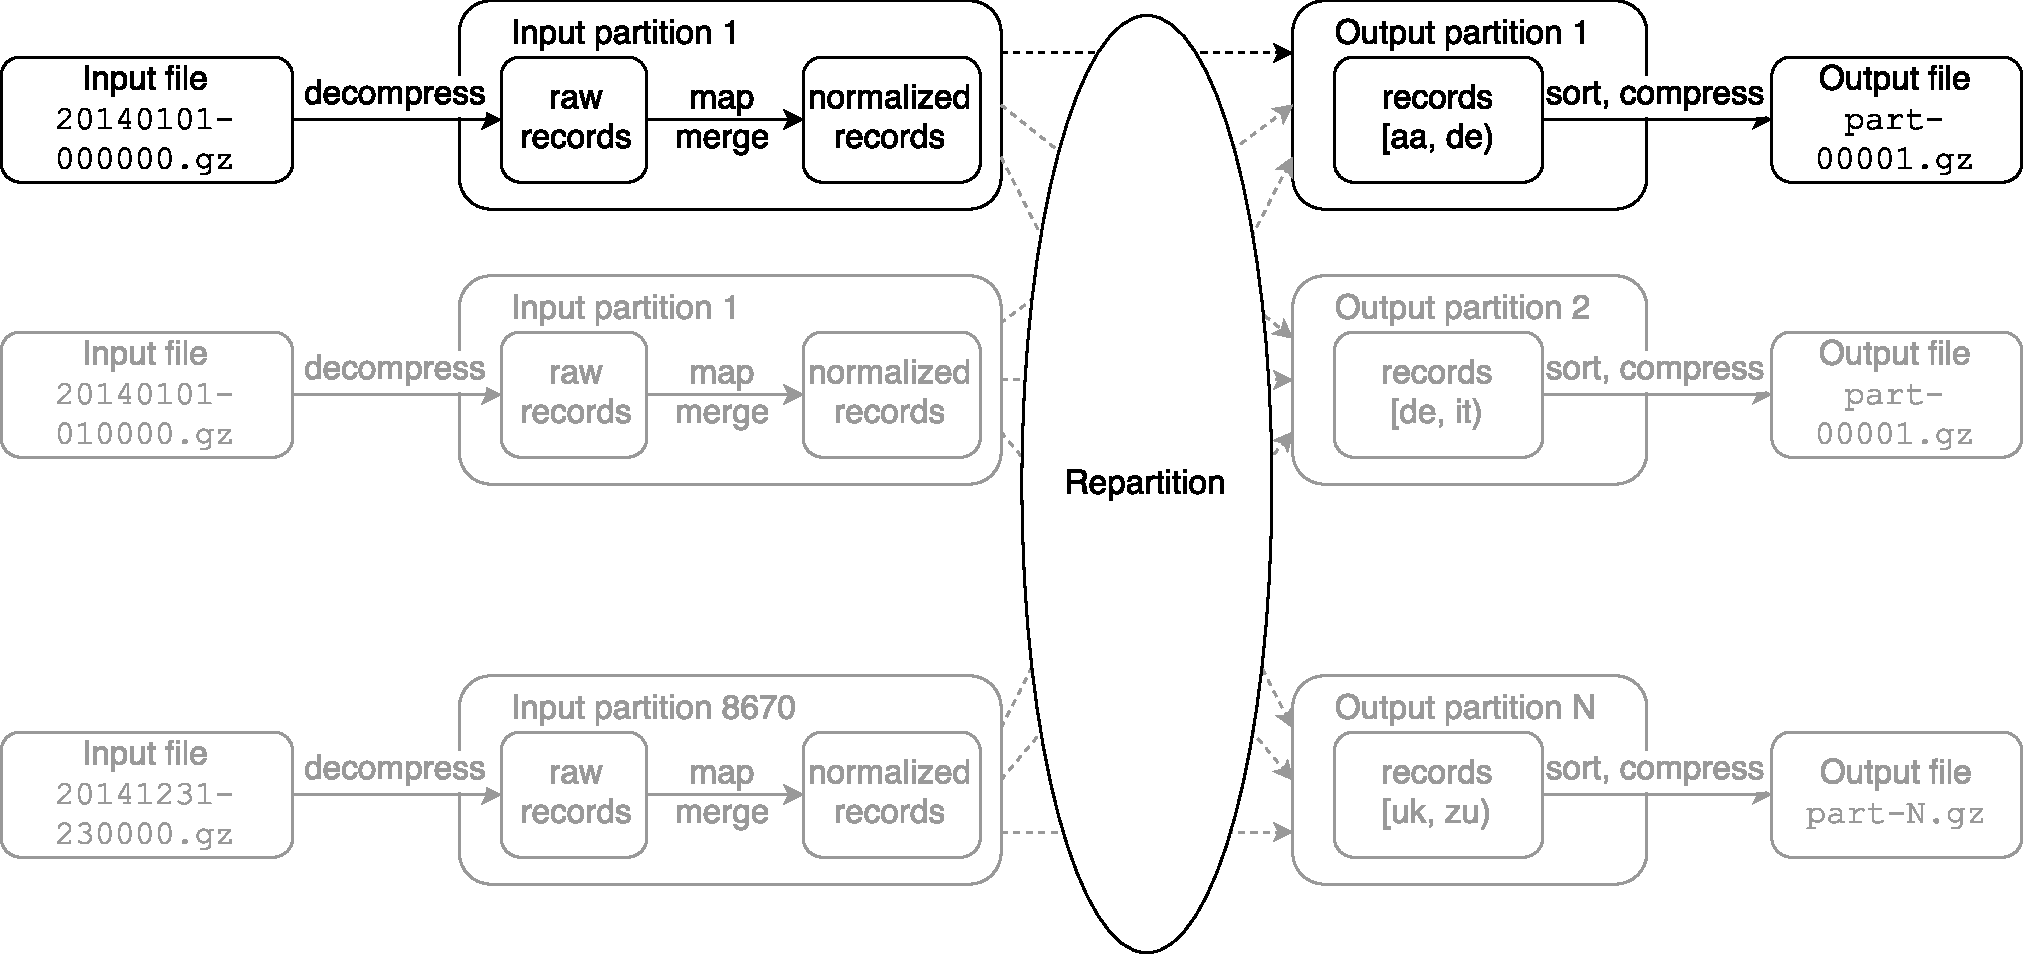
\includegraphics[width=0.9\textwidth]{assets/spark-pagecounts}
    \caption{Workflow showing the processing of Wikimedia page views}
    \end{figure}
\end{frame}


\section{Results}


% \begin{frame}{Quality of papers in Wikipedia}
% \begin{itemize}
%     \item Freshness of citations
%     \item Popularity of cited papers
%     \item Rank of cited journals
%     \item Lifetime of irrelevant citations
%     % \item Age of papers when inserted --- Freshness
%     % \item Incoming citations distribution
%     % \item Journals rank
%     % \item Lifetime of citations
% \end{itemize}
% \end{frame}

\subsection{Freshness of citations}
\begin{frame}{Age of papers when inserted}
    \begin{itemize}
        \item How old is a paper when it is inserted in Wikipedia for the first time?
        \item Exploit the DOI mapping with the Microsoft dataset
        \item Interesting behavior of papers having few days
    \end{itemize}
\end{frame}

\begin{frame}{Age of papers when inserted}
    \begin{figure}
    \centering
    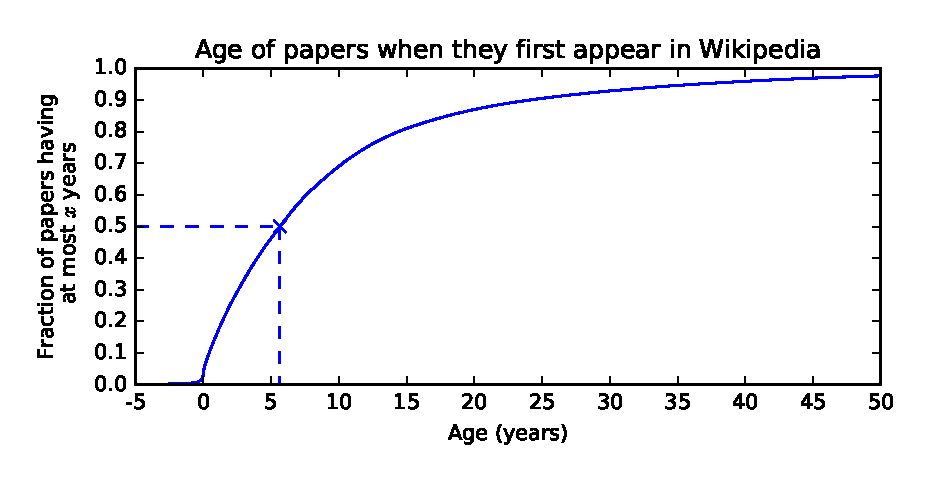
\includegraphics[width=0.9\textwidth]{assets/age_of_papers_at_first_appearance_cdf_slides}
    \end{figure}
    \begin{itemize}
        \item Half of the papers cited are less than 5.5 years old
    \end{itemize}
\end{frame}

\begin{frame}{Age of papers when inserted --- Detail}
    \begin{figure}
    \centering
    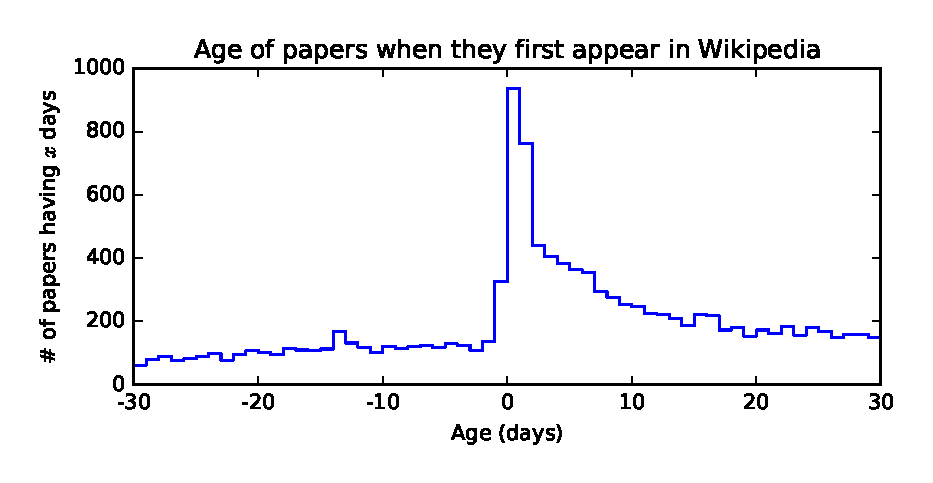
\includegraphics[width=0.9\textwidth]{assets/age_of_papers_at_first_appearance_pdf_near0_slides}
    \end{figure}
    \centering
    \begin{itemize}
        \item 1.3\% of papers are inserted within 7 days after the publication
    \end{itemize}
\end{frame}


\subsection{Popularity of cited papers}
\begin{frame}{Incoming citations distribution}
    \begin{columns}
        \column{0.3\textwidth}
        \begin{itemize}
            \item Arguably follows a power law~\cite{Redner1998}: $N(x) \sim x^{-\alpha}$
            \item How well papers in Wikipedia perform?
        \end{itemize}
        \column{0.7\textwidth}
        \begin{figure}
        \centering
        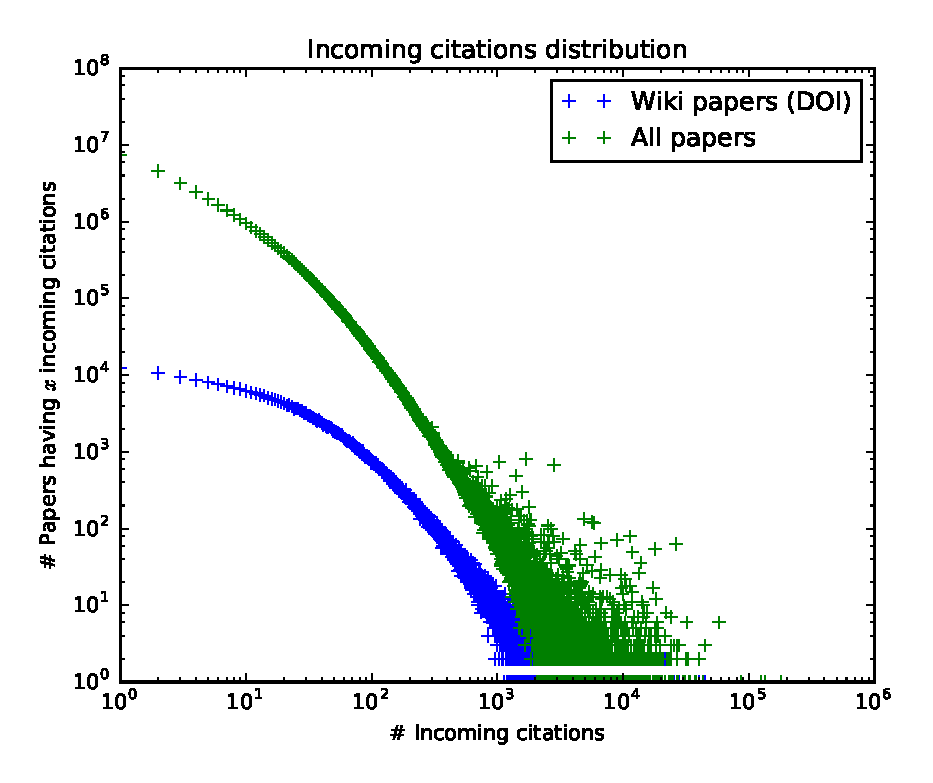
\includegraphics[width=1\textwidth]{assets/incoming_citations_distribution_pdf_slides}
        \end{figure}
    \end{columns}

\end{frame}

\begin{frame}{Incoming citations distribution}
    \begin{columns}
        \column{0.4\textwidth}
        \begin{itemize}
            \item Papers in Wikipedia behave like \emph{Genome Research} and \emph{PNAS}
            \item They outclass \emph{Nature} and \emph{Science}
            \item 74\% of papers in Wikipedia have more than 10 incoming citations
        \end{itemize}
        \column{0.6\textwidth}
        \begin{figure}
        \centering
        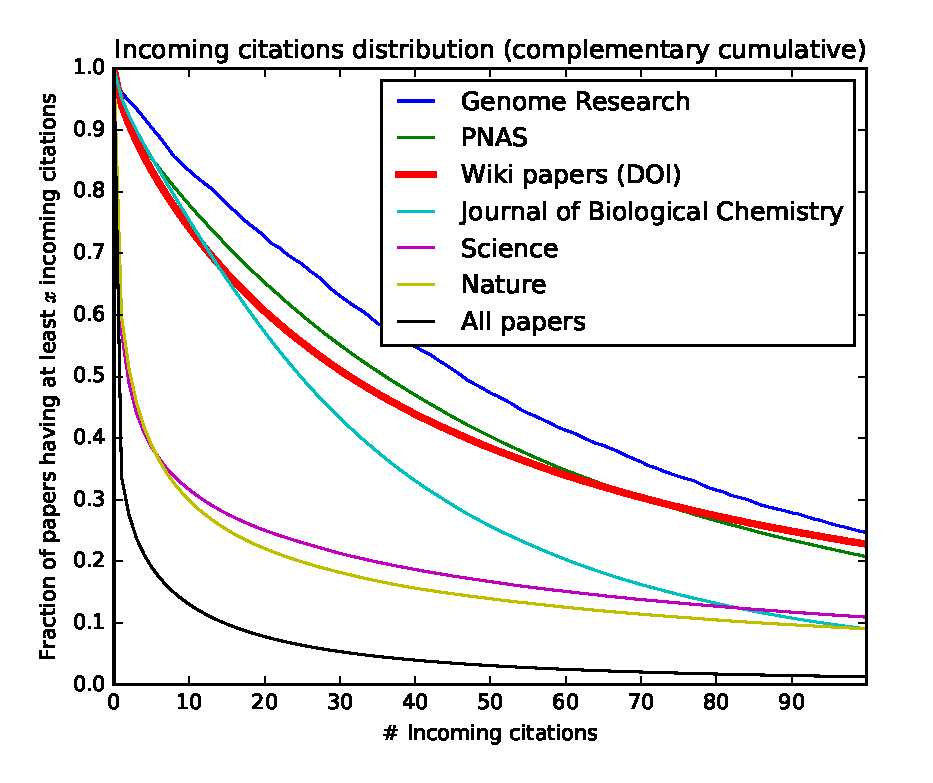
\includegraphics[width=1\textwidth]{assets/incoming_citations_distribution_ccdf_slides}
        \caption{Papers cited in Wikipedia vs papers in top journals}
        \end{figure}
    \end{columns}
\end{frame}

\subsection{Rank of cited journals}
\begin{frame}{Journals rank}
    \begin{itemize}
        \item First proposed by Nielsen in 2007~\cite{Nielsen2007}
        \item Most cited journals in Wikipedia are also the most important ones
        \item[]
        \item Journals rank by impact factor (from JCR) versus:
        \begin{itemize}
            \item citations in Wikipedia
            \item visualizations in Wikipedia (in 2014)
        \end{itemize}
        \item Measured in term of Kendall rank correlation coefficient ($-1 \le \tau \le 1$)
    \end{itemize}
\end{frame}

\begin{frame}{Journals impact factor vs Wikipedia citations}
    \begin{figure}
    \centering
    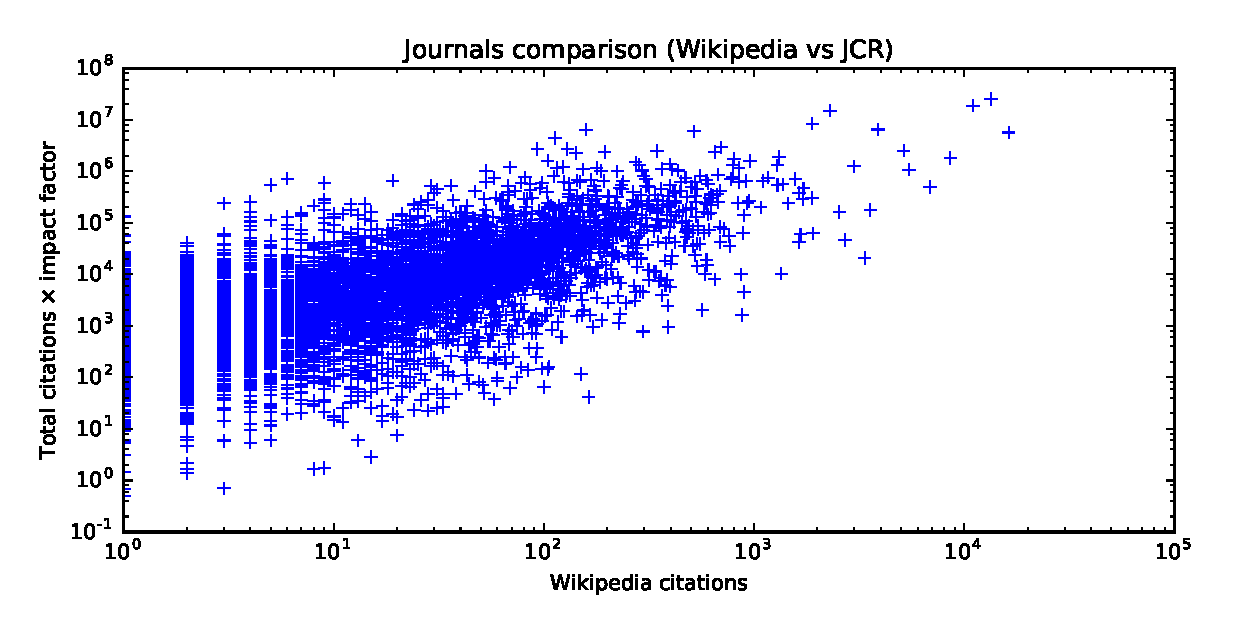
\includegraphics[width=0.9\textwidth]{assets/journals_compare_appearances}
    \end{figure}

    \begin{itemize}
        \item Kendall rank correlation coefficient: $0.464$
    \end{itemize}
\end{frame}

\begin{frame}{Journals impact factor vs Wikipedia impressions}
    \begin{figure}
    \centering
    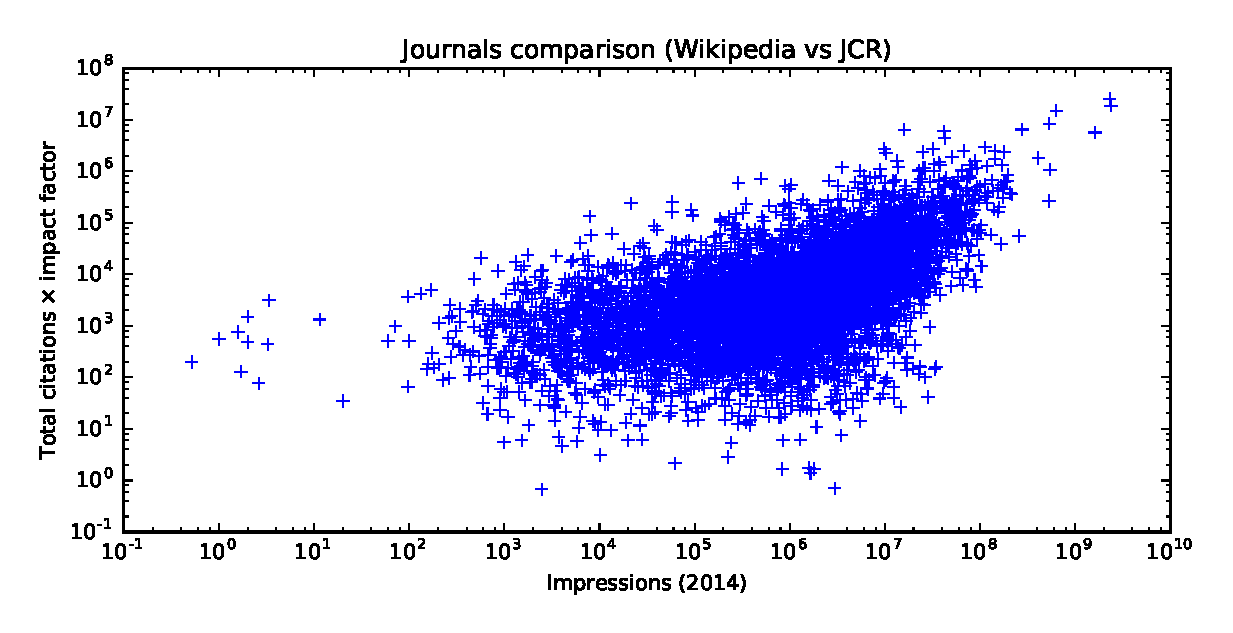
\includegraphics[width=0.9\textwidth]{assets/journals_compare_impressions2014}
    \end{figure}

    \begin{itemize}
        \item Kendall rank correlation coefficient: $0.401$
    \end{itemize}
\end{frame}
%
% \begin{frame}{Maybe: Journals citations vs impressions in Wikipedia}
%     \begin{figure}
%     \centering
%     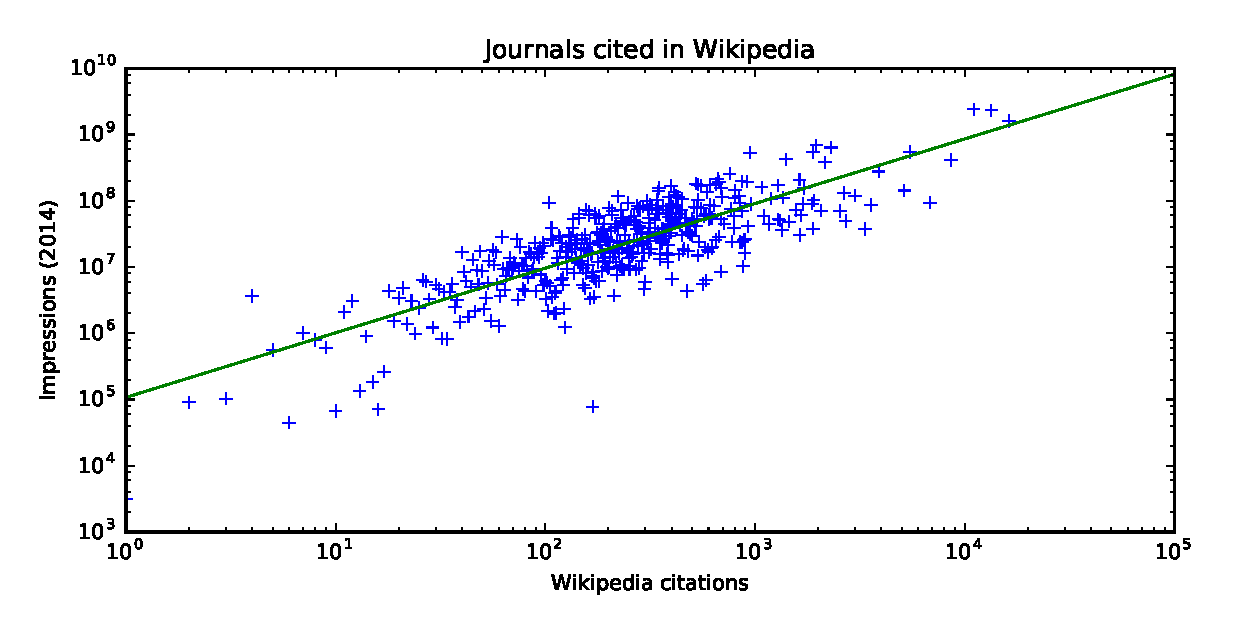
\includegraphics[width=0.9\textwidth]{assets/journals_appearances_impressions_loglog_slides}
%     \end{figure}
%     \centering
%     Linear regression model: $\hat{y}_i = 10^{5.03} \times x^{0.98}$ ($r^2=0.65$)
% \end{frame}

\subsection{Lifetime of irrelevant citations}
\begin{frame}{Lifetime of irrelevant citations}
    \begin{itemize}
        \item How long does it take for a Wikipedia contributor to discover and remove an ``irrelevant'' paper from an article?
        \item A paper is ``irrelevant'' for an article if it appeared on that page and was then removed.
    \end{itemize}
\end{frame}

\begin{frame}
    \begin{columns}[c]
        \column{0.5\textwidth}
        \begin{itemize}
            \item Fraction of papers removed in time % (970\,273 in total)
            \item[]
            \item 61\% of irrelevant DOI removed within one year
            \item 36\% within one month
            \item 24\% within one day
        \end{itemize}
        \column{0.5\textwidth}
        \begin{figure}
        \centering
        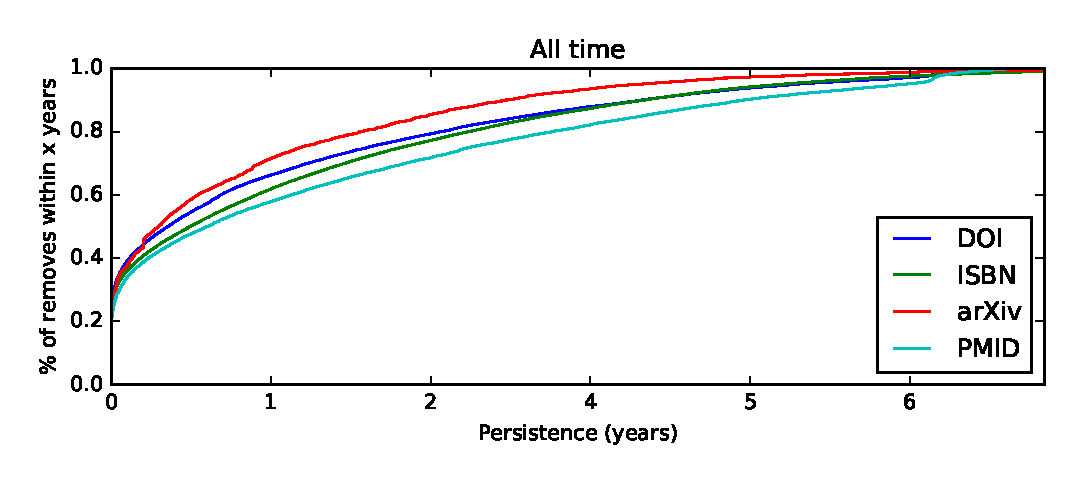
\includegraphics[width=1\textwidth]{assets/irrelevant_identifiers_persistence_cdf_max_slides}

        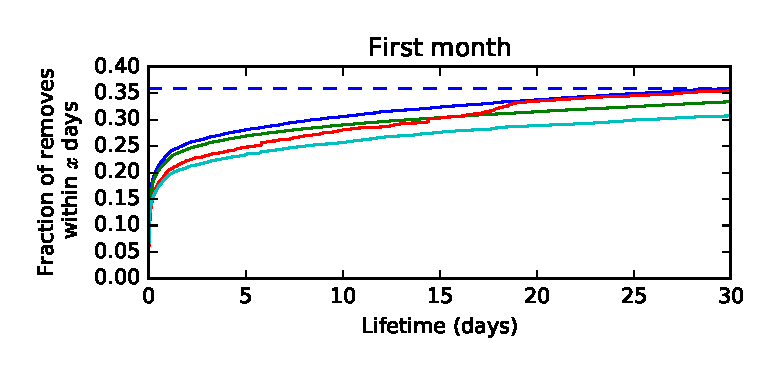
\includegraphics[width=1\textwidth]{assets/irrelevant_identifiers_persistence_cdf_1month_slides}

        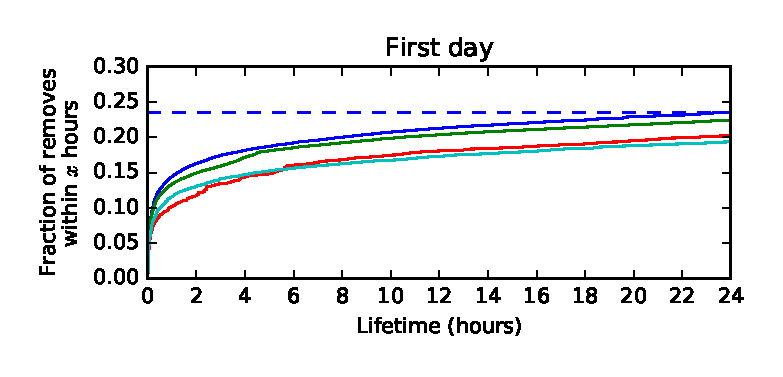
\includegraphics[width=1\textwidth]{assets/irrelevant_identifiers_persistence_cdf_1day_slides}
        \end{figure}
    \end{columns}
\end{frame}

\section{Further work}

\begin{frame}{Further work}
    \begin{itemize}
        \item Exploit the page views dataset and the framework
        \item Open questions:
        \begin{itemize}
            \item If a paper appears in Wikipedia, will it become more popular in the scientific community?
            \item In another way, do researcher use Wikipedia as their primary data source?
            \item Predict whether a publication is going to stay on a page
        \end{itemize}
    \end{itemize}
\end{frame}

\appendix

\begin{frame}[allowframebreaks,noframenumbering]{References}
    \bibliographystyle{plain}
    \bibliography{biblio}
\end{frame}


\end{document}
